\section{Walks}

\frame{
{Part 2: Walks in Graphs}

\tableofcontents[currentsection,hideallsubsections, firstsection=1, sections={1-4}]
}

\subsection{Walks, Paths and Relations}

\begin{frame}{Walks and Paths}

  The example of the "course schedule" shows that the solution of a problem can be represented as a sequence of vertices or edges.\bigskip

  We can talk about these sequences as "Walks" or "Paths".\bigskip

  \begin{itemize}
    \item A {\bf Walk} is a sequence of successive edges;\bigskip

    \item A {\bf Path} is a walk that does not repeat vertices;
  \end{itemize}
\end{frame}

\begin{frame}{Walk example}

  \begin{center}
    \begin{tikzpicture}[scale=1.5,auto,swap]
      \tikzset{edge/.style = {->,>=latex'}}
      \node[vertex] (a) at (0,1) {a};
      \node[vertex] (b) at (0,0) {b};
      \node[vertex] (c) at (0,-1) {c};
      \node[vertex] (d) at (2,0) {d};
      \node[vertex] (e) at (3,1) {e};
      \node[vertex] (f) at (3,-1) {f};
      \draw[edge] (a) to (b);
      \draw[edge] (c) to (b);
      \draw[edge] (b) to (d);
      \draw[edge] (d) to (a);
      \draw[edge] (c) to (d);
      \draw[edge] (d) to (e);
      \draw[edge] (e) to (f);
      \draw[edge] (f) to (d);
  \end{tikzpicture}
  \end{center}

  \bigskip

  \begin{block}{Walk: a sequence of successive edges}

    \begin{tikzpicture}[scale=1,auto,swap]
      \tikzset{edge/.style = {->,>=latex'}}
      \node[vertex] (a) at (0,0) {b};
      \node[vertex] (b) at (1,0) {d};
      \node[vertex] (c) at (2,0) {e};
      \node[vertex] (d) at (3,0) {f};
      \node[vertex] (e) at (4,0) {d};
      \node[vertex] (f) at (5,0) {e};
      \draw[edge] (a) to (b);
      \draw[edge] (b) to (c);
      \draw[edge] (c) to (d);
      \draw[edge] (d) to (e);
      \draw[edge] (e) to (f);
    \end{tikzpicture}

    \begin{itemize}
    \item {\bf Walk lengh:} 5 edges (The length of a walk is the EDGES, not the VERTICES)
    \item {\bf Representing as a relation:} $E(E(E(E(E(a)))))$
    \item Note that a walk can repeat edges and vertices! It is just a compound relation.
    \end{itemize}
  \end{block}

\end{frame}

\begin{frame}
  \frametitle{Path example}

  \begin{center}
    \begin{tikzpicture}[scale=1.5,auto,swap]
      \tikzset{edge/.style = {->,>=latex'}}
      \node[vertex] (a) at (0,1) {a};
      \node[vertex] (b) at (0,0) {b};
      \node[vertex] (c) at (0,-1) {c};
      \node[vertex] (d) at (2,0) {d};
      \node[vertex] (e) at (3,1) {e};
      \node[vertex] (f) at (3,-1) {f};
      \draw[edge] (a) to (b);
      \draw[edge] (c) to (b);
      \draw[edge] (b) to (d);
      \draw[edge] (d) to (a);
      \draw[edge] (c) to (d);
      \draw[edge] (d) to (e);
      \draw[edge] (e) to (f);
      \draw[edge] (f) to (d);
  \end{tikzpicture}
  \end{center}

  \begin{block}{Path: A walk without repeated vertices}

    \begin{tikzpicture}[scale=1,auto,swap]
      \tikzset{edge/.style = {->,>=latex'}}
      \node[vertex] (a) at (0,0) {e};
      \node[vertex] (b) at (1,0) {f};
      \node[vertex] (c) at (2,0) {d};
      \node[vertex] (d) at (3,0) {a};
      \node[vertex] (e) at (4,0) {b};
      \draw[edge] (a) to (b);
      \draw[edge] (b) to (c);
      \draw[edge] (c) to (d);
      \draw[edge] (d) to (e);
    \end{tikzpicture}\hspace{1cm} {\bf Stuck!}

    \begin{itemize}
    \item {\bf Walk lengh:} 4 edges (Not 5 vertices)
    \item Can you find a walk that visits all vertices in the graph?
    \end{itemize}
  \end{block}
\end{frame}

\begin{frame}{Walks and Paths}
  Simple example proof with graphs: \emph{"The shortest walk between two vertices is a Path"}

  \begin{proof}
    {\bf Proof by contradiction:} Assume a shortest walk that is not a graph.

    \begin{enumerate}
    \item The shortest walk between $v_0$ and $v_n$ is not a path. So it has a repeated vertice $v_k$:
    \begin{equation*}
      w_s = v_0 \to v_1 \to \ldots \to v_k \to \ldots \to v_k \to \ldots \to v_{n-1} \to v_n
    \end{equation*}

    \item The walk $w_s$ from $v_0$ to $v_n$, contains a small walk $w_k$ from $v_k$ to $v_k$ of size $|w_k| \geq 1$.
    \item We can remove $w_k$ from $w_s$, resulting in a smaller walk $w_s'$ with size $|w_s| - |w_k|$
    \item $w_s'$ is a walk from $v_0$ to $v_n$ that is shorter than $w_s$, which is a contradiction.
    \end{enumerate}
  \end{proof}

\end{frame}

\begin{frame}{The Walk Relation}

  We define the \structure{Length $n$ Walk Relation}:
  \begin{equation}
    v G^n w.
  \end{equation}\bigskip

  This means "There is a walk of length exactly $n$ from $v$ to $w$ in $G$".\bigskip

  Some facts about the $G^n$
  \begin{itemize}
  \item $G^1$ is the relation of vertices directly connected by edges in $G$.
  \item {\bf addition:} $G^n \circ G^m = G^{n+m}$ \hspace{.5cm}
    (the composite of two Walk Relations is their addition)
  \item {\bf common vertex:} $x~G^m \circ G^n~y \rightarrow \exists z, x~G^m~z~G^n~y$
    \hfill ($G^m\circ G^n$ has a common vertex)
  \end{itemize}
\end{frame}

\begin{frame}{Walk Relations: Composition and the Adjacency Matrix}

  Consider the adjency matrix $A_{G^n}$ that describes the relation $G^n$: $a_{ij} = 1 \iff v_i G v_j$.\bigskip

  It is possible to calculate the Adjacency Matrix of a composite walk relation using \emph{boolean matrix multiplication}: $A_{G^n\circ G^m} = A'_{G^n} \odot A''_{G_m}$:

  \begin{equation}
    a_{ij} = A'_{i*} \odot A''_{*j} = (a'_{i0} \land a''_{0j}) \lor (a'_{i1} \land a''_{1j}) \lor (a'_{i2} \land a''_{2j}) \lor \ldots \lor (a'_{in} \land a''_{nj})
  \end{equation}\bigskip

  This means that we can calculate $A_{G^n}$ quickly using the \structure{Fast Matrix Exponentiation} algorithm:

  \begin{itemize}
    \item $A_{G^n} = A_{G^{n/2}} \odot A_{G^{n/2}} = (A_{G^{n/4}} \odot A_{G^{n/4}}) \odot (A_{G^{n/4}} \odot A_{G^{n/4}}) = \ldots$
  \end{itemize}

\end{frame}

\begin{frame}
  \frametitle{Walk Relation $G^*$ of a Digraph}

  \begin{itemize}
  \item $G^n$ is the \structure{length $n$ walk relation}; while $G^*$ is the \structure{walk relation of $G$}
  \item $u G^* v$ means that there is a walk from $u$ to $v$ \structure{of {\bf any} length}\\
  \end{itemize}\bigskip

  \alert{QUIZ:} How do we calculate $G^*$ for a graph, given the adjacency matrix $A$?\bigskip

  Remember that a walk can be infinite. So is it possible to solve this problem with a {\bf finite} algorithm?
\end{frame}

\begin{frame}{Walk Relation of a DiGraph}{How to calculate $G^*$}

  \begin{enumerate}
  \item Let $G^1$ be the relation defined by the original graph (or its adjacency matrix).\medskip

  \item Let $G^0$ be the relation defined by the set $V$ with self:
    \begin{tikzpicture}[scale=1.5,auto,swap]
      \tikzset{edge/.style = {->,>=latex'}}
      \node[vertex] (a) at (0,0) {};
      \draw[edge] (a) to[loop left] (a);
    \end{tikzpicture} (Or the identity matrix).\medskip

  \item The relation $G^{\leq 1} = G^0 \cup G^1$ is the relation for walks of \emph{length 1 or less};\medskip

  \item $G^* = (G^{\leq})^{n-1}$, so you can calculate $G^*$ in $\log n$ matrix boolean multiplications
  \end{enumerate}
\end{frame}

\begin{frame}{Walks and Prerequisite Course Graphs}
  \begin{columns}
    \column{0.4\textwidth}
      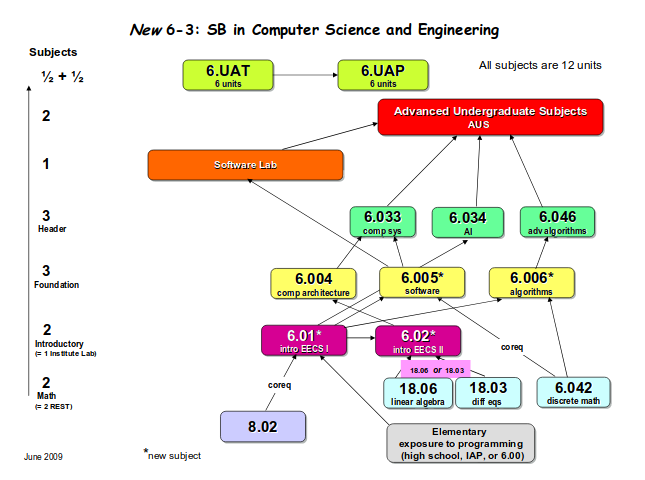
\includegraphics[width=1\textwidth]{../img/MIT_prereq}
      \pagenote{Course Pre-requisite image from "Math for CS" MIT OCW}
    \column{0.6\textwidth}
      The \emph{walk relation} of the pre-requisite graph $R$ defines how the courses relate to each other.
      \begin{itemize}
      \item \structure{Direct Prerequisite}: Req(6.046) = 6.006
      \item \structure{Indirect Prerequisite}: Req(6.046) = $\{6.006, 6.042, 6.01, 6.00, 8.02\}$
      \end{itemize}\medskip
  \end{columns}\bigskip

  Course $u$ is an indirect prerequisite of $v$ if there is a positive length walk from $u$ to $v$ in $R$:\medskip

  \begin{equation*}
    u D^+ v
  \end{equation*}
\end{frame}

\begin{frame}
  \frametitle{Requisites, Cycles and DAGs}

  In the beginning of the lecture, we talked about a prerequisite graph where it was not possible to graduate. Why? Because it had {\bf cycles}.\medskip

    \begin{itemize}
    \item A \structure{closed walk} is a walk that starts and ends at the same vertex.\medskip

    \item A \structure{cycle} is a closed walk where the only repeat
      vertex is at the beginning and end.
      \begin{itemize}
        \item $v_0 \to v_1 \to \ldots \to v_n \to v_0 | i > 0, j > 0, v_i \neq v_j$
        \item A cycle is the path $v \to w + (w,v)$
      \end{itemize}\medskip

    \item A \alert{Directed Acyclic Graph (DAG)} is a digraph that has
      \structure{no positive length cycles}.
    \end{itemize}
\end{frame}

\begin{frame}{Directed Acyclic Graphs Examples}

  Directed Acyclic Graphs (DAGs), can be used to represent several ordered structures:

    \begin{itemize}
      \item Course Prerequisite Graphs;
      \item Ordered Task List:
      \begin{itemize}
        \item "first add rice, then add water, then press cook button"
        \item "Let x be 5, let y be 2, while y $>$ 0, multiply x by x and subtract 1 from y."
      \end{itemize}
    \end{itemize}
    \bigskip

  Computational structures can also be described using DAGs:\medskip

    \begin{itemize}
      \item Relations, for example:
      \begin{itemize}
        \item \structure{Successor Relation}: $n \to n+1$
        \item \structure{Subset Relation}: $\{1,2\} \subset \{1,2,3\}$
      \end{itemize}
      \item Induction Proofs: ($P(n) \implies P(n+1) \implies P(n+2) \ldots$);
      \item Dynamic Programming: (base cases and transitions on the DP table);
    \end{itemize}
\end{frame}

\begin{frame}
  \frametitle{Directed Acyclic Graphs (DAG) and covering edges}

  \begin{columns}
    \column{0.3\textwidth}
    \begin{tikzpicture}[scale=.5,auto,swap]
      \tikzset{edge/.style = {->,>=latex'}}
      \node[vertex] (a) at (2,5) {a};
      \node[vertex] (b) at (1,3) {b};
      \node[vertex] (c) at (3,3) {c};
      \node[vertex] (d) at (2,2) {d};
      \node[vertex] (e) at (0,0) {e};
      \node[vertex] (f) at (4,0) {f};
      \draw[edge] (a) to (b);
      \draw[edge] (a) to (c);
      \draw[edge] (a) to (d);
      \draw[edge] (c) to (f);
      \draw[edge] (d) to (f);
      \draw[edge] (c) to (d);
      \draw[edge] (b) to (d);
      \draw[edge] (a) to[bend right] (e);
      \draw[edge] (a) to[bend left] (f);
      \draw[edge] (b) to[bend right] (f);
    \end{tikzpicture}

    \begin{tikzpicture}[scale=.5,auto,swap]
      \tikzset{edge/.style = {->,>=latex'}}
      \node[vertex] (a) at (2,5) {a};
      \node[vertex] (b) at (1,3) {b};
      \node[vertex] (c) at (3,3) {c};
      \node[vertex] (d) at (2,2) {d};
      \node[vertex] (e) at (0,0) {e};
      \node[vertex] (f) at (4,0) {f};
      \draw[edge] (a) to (b);
      \draw[edge] (a) to (c);
      \draw[edge] (d) to (f);
      \draw[edge] (c) to (d);
      \draw[edge] (b) to (d);
      \draw[edge] (a) to[bend right] (e);
    \end{tikzpicture}

    \column{0.7\textwidth}

      Given a DAG $A$, its \structure{covering edges} is the {\bf smallest} DAG $B$ that has the same \structure{Walk Relation} as $A$\bigskip

      Walk relation of $A$ and $B$:
      \begin{itemize}
      \item $a\to \{b,c,d,e,f\}$
      \item $\{b,c\}\to \{d,f\}$
      \item $d\to f$
      \item $\{e,f\} \to \emptyset$
      \end{itemize}
  \end{columns}
\end{frame}
